\documentclass[11pt,letterpaper]{article}

% Load some basic packages that are useful to have
% and that should be part of any LaTeX installation.
%
% be able to include figures
\usepackage{graphicx}
% get nice colors
\usepackage{xcolor}

% change default font to Palatino (looks nicer!)
\usepackage[latin1]{inputenc}
\usepackage{mathpazo}
\usepackage[T1]{fontenc}
% load some useful math symbols/fonts
\usepackage{latexsym,amsfonts,amsmath,amssymb}

% comfort package to easily set margins
\usepackage[top=1in, bottom=1in, left=1in, right=1in]{geometry}

% control some spacings
%
% spacing after a paragraph
\setlength{\parskip}{.15cm}
% indentation at the top of a new paragraph
\setlength{\parindent}{0.0cm}


\begin{document}

\begin{center}
\Large
Ay190 -- Worksheet 14\\
John Pharo\\
Date: \today\\
Bruce Willis' Stunt Double: Matthias Raives
\end{center}

\section*{Advection and Shocks}

Below are plots of the function 

$$ \Psi = \frac{1}{8}\sin \left( \frac{2 \pi x}{L} \right) $$

evolved through time. $L=100$, and $x \in [0,100]$. Below the plots of the functions are plots of the size of the time step as a function of time. I also plotted the analytical solution in red, just because it was already in the code, though it doesn't seem especially useful here.

\begin{figure}[bth]
\centering
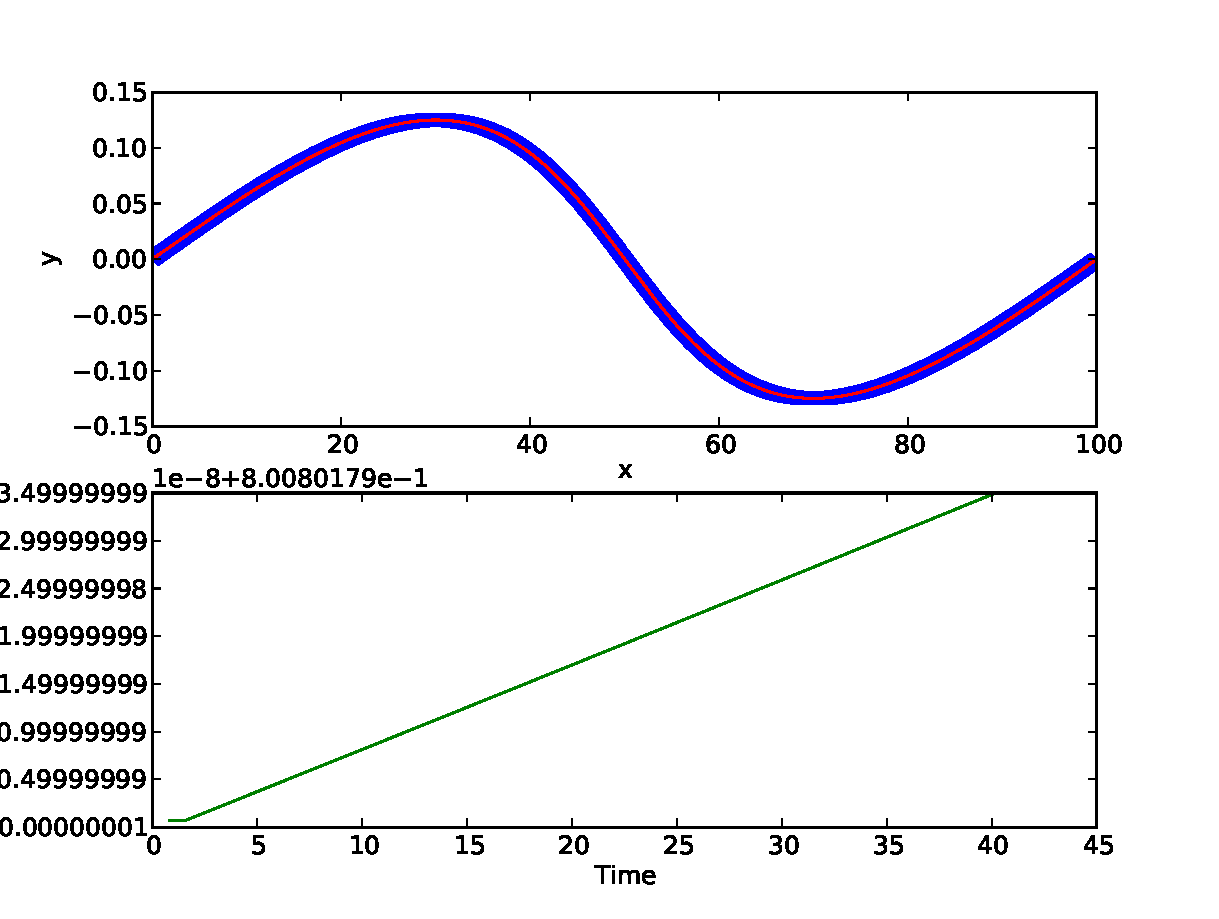
\includegraphics[width=0.5\textwidth]{t=50.pdf}
\caption{This is a plot of the function at t=50.}
\label{fig:simpleplot2}
\end{figure}

\begin{figure}[bth]
\centering
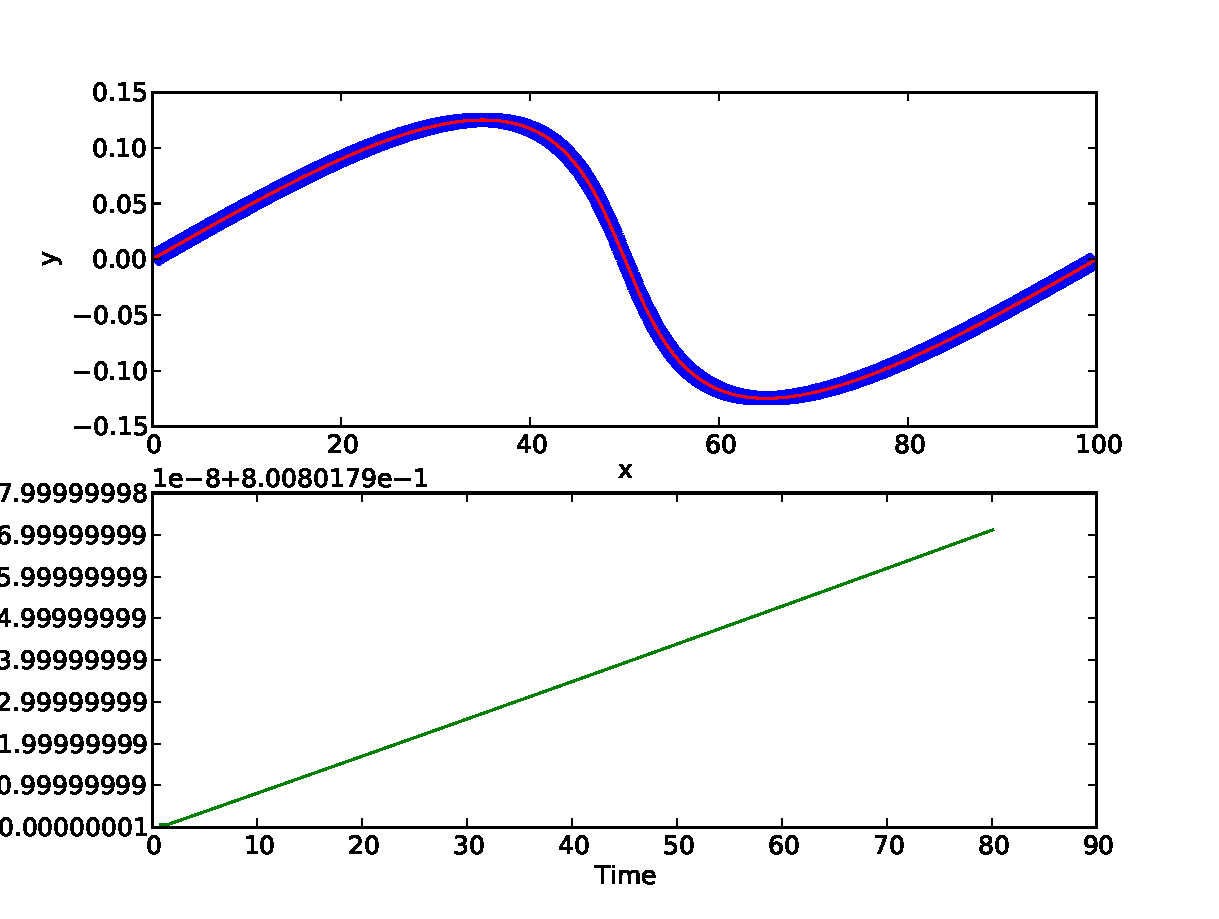
\includegraphics[width=0.5\textwidth]{t=100.pdf}
\caption{This is a plot of the function at t=100.}
\label{fig:simpleplot2}
\end{figure}

\begin{figure}[bth]
\centering
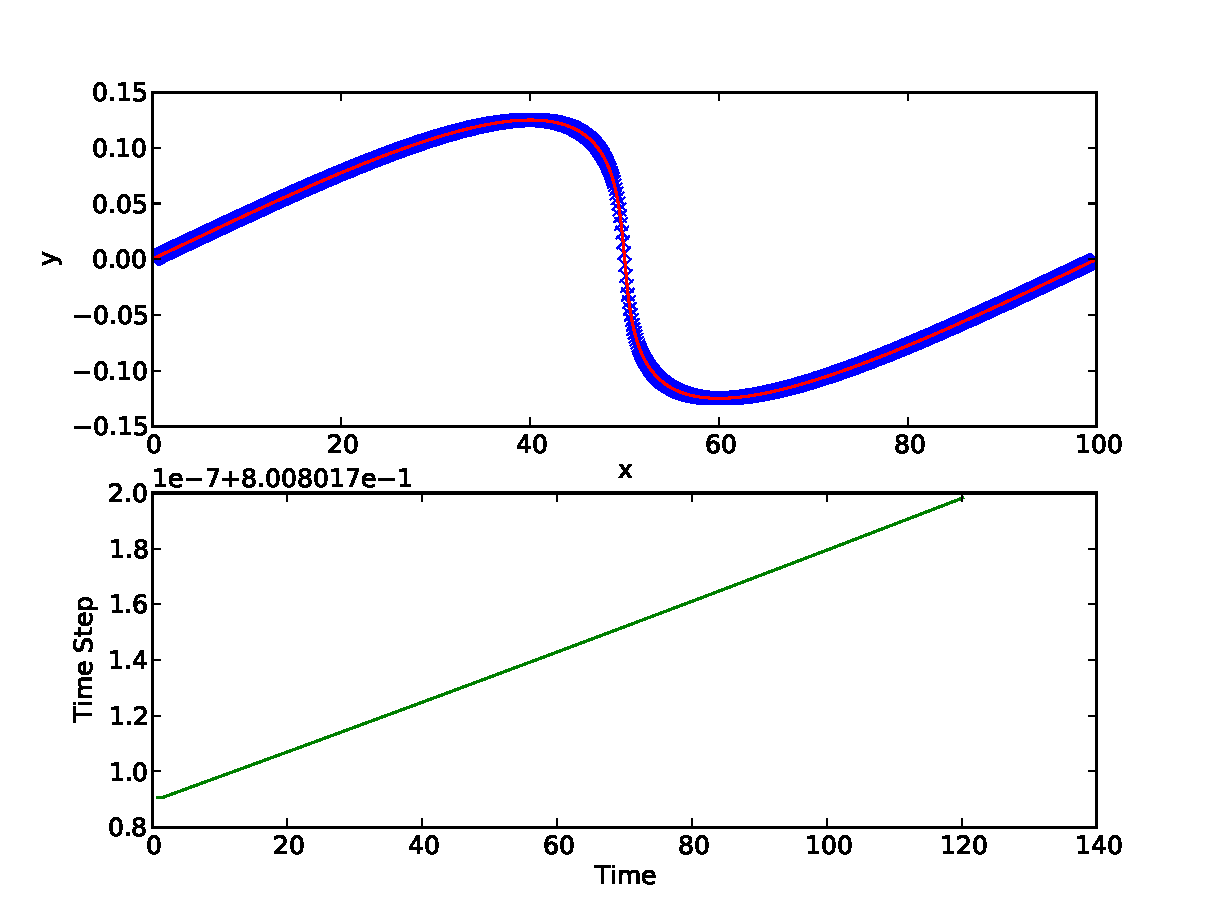
\includegraphics[width=0.5\textwidth]{t=150.pdf}
\caption{This is a plot of the function at t=150. You can begin to see the formation of the shock as the peaks get closer.}
\label{fig:simpleplot2}
\end{figure}

\begin{figure}[bth]
\centering
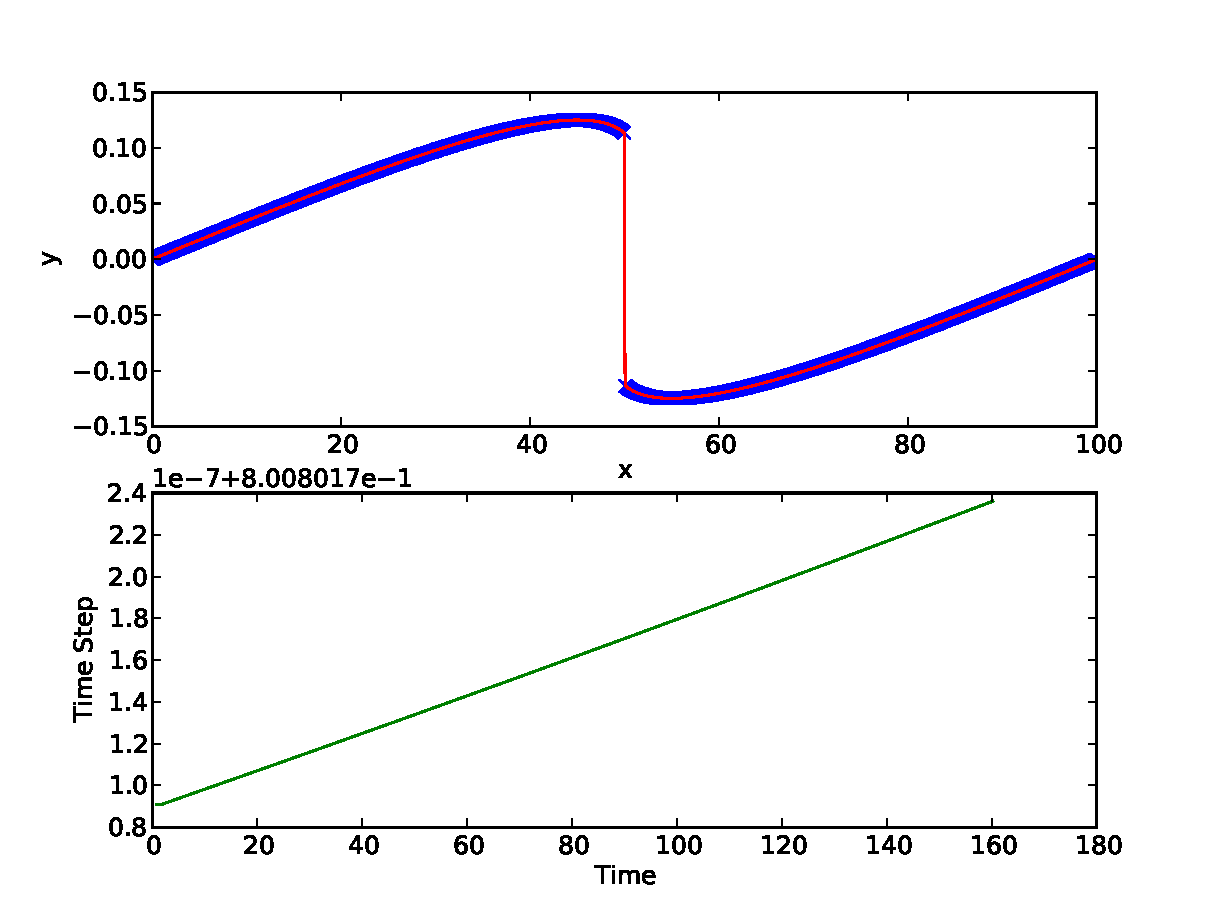
\includegraphics[width=0.5\textwidth]{t=200.pdf}
\caption{This is a plot of the function at t=200. By now the shock has fully formed.}
\label{fig:simpleplot2}
\end{figure}


\end{document}
